% Authors: Greg Westphal and Kathryn Huff
\documentclass[border=10pt]{standalone}
\usepackage{tikz}
\usetikzlibrary{arrows.meta}
\tikzset{%
  >={Latex[width=2mm,length=2mm]},
  % Specifications for style of nodes:
            base/.style = {rectangle, rounded corners, draw=black,
                           minimum width=3cm, minimum height=1cm,
                           text centered, font=\sffamily},
       bluebox/.style = {base, fill=gray!15}, %blue!30
       redbox/.style = {base, fill=white!30}, %red
       greenbox/.style = {base, fill=white!30}, %green
       process/.style = {base, minimum width=2.5cm, fill=gray!30, %orange!15
                           font=\ttfamily},
}
% Drawing part, node distance is 1.5 cm and every node
% is prefilled with white background
\begin{document}
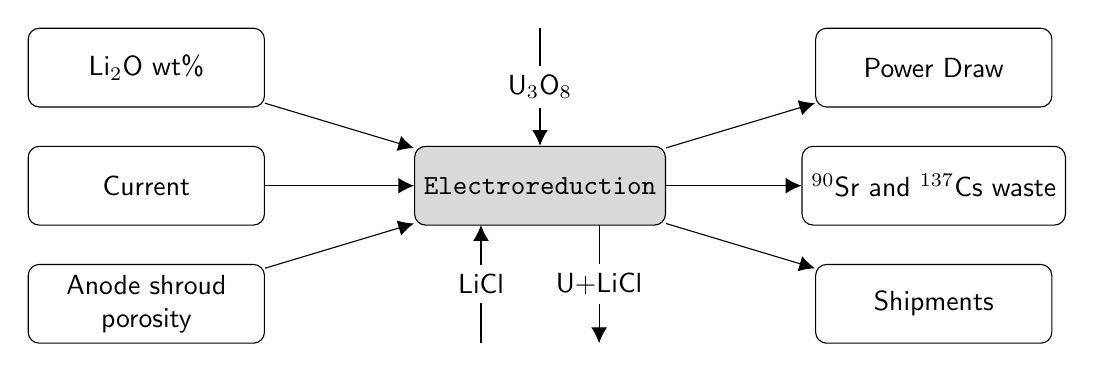
\begin{tikzpicture}[node distance=3cm,
    every node/.style={fill=white, font=\sffamily}, align=center]
  % Specification of nodes (position, etc.)
  
 
  \node (reduction)			[process] {Electroreduction};
  \node (decay)				[redbox, right of=reduction, xshift=2cm] {$^{90}$Sr and $^{137}$Cs waste};
  \node (Li2O)	 			[greenbox, left of=reduction, xshift=-2cm, yshift=1.5cm] {Li$_2$O wt\%};
  \node (current)	 		[greenbox, left of=reduction, xshift=-2cm] {Current};
  \node (porosity)			[greenbox, left of=reduction, xshift=-2cm, yshift=-1.5cm] {Anode shroud \\ porosity};
  \node (power)				[redbox, right of=reduction, xshift=2cm, yshift=1.5cm] {Power Draw};
  \node (shipments)			[redbox, right of=reduction, xshift=2cm, yshift=-1.5cm] {Shipments};
  
  \draw[->]					(reduction) -- (power);
  \draw[->]					(reduction) -- (shipments);
  \draw[->]					(reduction) -- (decay);
  \draw[->]					(Li2O) -- (reduction);
  \draw[->]					(porosity) -- (reduction);
  \draw[->]					(current) -- (reduction);
  \draw[->]					(reduction)++(0,2) -- (reduction) node[midway] {U$_3$O$_8$};
  \draw[->]					(reduction)++(-0.75,-2) -- ++(0,1.5) node[midway] {LiCl};
  \draw[->]					(reduction)++(0.75,-0.5) -- ++(0,-1.5) node[midway] {U+LiCl};

  \end{tikzpicture}
\end{document}